\section{Introduction}
\label{sec:intro}

The effective reproduction number is defined to be the average number of
secondary infections caused by a primary infection that occurred sometime in the past. 
Also called the instantaneous reproduction number, it is a key quantity
for understanding infectious disease dynamics including the potential size of an
outbreak and the required stringency of control measures.  Tracking the time
series of this quantity is useful for understanding whether or not
future infections are likely to increase or decrease from the current state. Let
$\calR(t)$ denote the effective reproduction number at time $t$. Practically, as
long as $\calR(t) < 1$, infections will decline gradually, eventually resulting
in a disease-free equilibrium, whereas when $\calR(t) > 1$, infections will
continue to increase, resulting in endemic equilibrium. While $\calR(t)$ is
fundamentally a continuous time quantity, it can be related to data only at
discrete points in time $t = 1,\ldots,n$. This sequence of effective
reproduction numbers over time is not observable, but, nonetheless, is easily
interpretable and retrospectively describes the course of an epidemic.
Therefore, a number of procedures exist to estimate $\calR_t$ from different
types of observed incidence data such as cases, deaths, or hospitalizations,
while relying on various domain-specific assumptions. Importantly, accurate
estimation of effective reproduction numbers relies heavily on the quality of
the available data, and, due to the limitations of data collection, such as
underreporting and lack of standardization, estimation methodologies rely on
various assumptions to compensate. Because model assumptions may not be easily
verifiable from data alone, it is also critical for any estimation procedure to
be robust to model misspecification. 


Many existing approaches for effective reproduction number estimation are
Bayesian: they estimate the posterior distribution of $\calR_t$ conditional on
the observations. One of the first such approaches is the software \EpiEstim\
\citep{cori2020package}, described in \cite{cori2013new}. This method is
prospective, in that it uses only observations available up to time $t$ in order
to estimate $\calR_t$ for each $i = 1,\ldots, t$. An advantage of \EpiEstim\ is
its straightforward statistical model: new incidence data follows the Poisson
distribution conditional on past incidence combined with the conjugate gamma
prior distribution for $\calR_t$ with fixed hyperparameters. Additionally, the
serial interval distribution, the distribution of the period between onsets of
primary and secondary infections in a population, is fixed and known. For this
reason, \EpiEstim\ requires little domain expertise for use, and it is
computationally fast. \cite{thompson2019improved} modified this method to
distinguish imported cases from local transmission and simultaneously estimate
the serial interval distribution. \cite{nash2023estimating} further extended
\EpiEstim\ by using ``reconstructed'' daily incidence data to handle irregularly
spaced observations. Recently, \cite{abbott2020estimating} proposed a Bayesian
latent variable framework, \texttt{EpiNow2} \citep{EpiNow2}, which leverages
incident cases, deaths or other available streams simultaneously along with
allowing additional delay distributions (incubation period and onset to
reporting delays) in modelling.  
\cite{lison2023generative} proposed an extension that handles missing data by
imputation followed by a truncation adjustment. These modifications are intended
to increase accuracy at the most recent (but most uncertain) timepoints, to aid 
policymakers. \cite{parag2021improved} also proposed a Bayesian approach, 
\texttt{EpiFilter} based on the (discretized) Kalman filter and smoother. 
\texttt{EpiFilter} also estimates the posterior of $\calR_t$ given a Gamma 
prior and Poisson distributed incident cases. Compared to \EpiEstim, 
however, \texttt{EpiFilter} estimates $\calR_t$ retrospectively using all 
available incidence data both before and after time $t$, with the goal of being 
more robust in low-incidence periods. \cite{gressani2022epilps} proposed a 
Bayesian P-splines approach, \EpiLPS, that assumes negative Binomial distributed 
observations. \cite{trevisin2023spatially} also proposed a Bayesian model estimated 
with particle filtering to incorporate spatial structures. 
Bayesian approaches estimate the posterior distribution of the effective
reproduction numbers and possess the advantage that credible intervals may be
easily computed. A limitation of many Bayesian approaches, however, is that they
usually require more intensive computational routines, especially when observed
data sequences are long or hierarchical structures are complex.  Below, we
compare our method to two of the more computationally efficient Bayesian models,
\EpiEstim\ and \EpiLPS. 


There are also frequentist approaches for $\calR_t$ estimation.
\cite{abry2020spatial} proposed regularizing the smoothness of $\calR_t$ through
penalized regression with second-order temporal regularization, additional
spatial penalties, and with Poisson loss. \cite{pascal2022nonsmooth} extended
this procedure by introducing another penalty on outliers.
\cite{pircalabelu2023spline} proposed a spline-based model relying on the
assumption of exponential-family distributed incidence. \cite{ho2023accounting}
estimates $\calR_t$ while monitoring the time-varying level of overdispersion.
There are other spline-based approaches such as
\cite{azmon2014estimation,gressani2021approximate}, autoregressive models with
random effects \citep{jin2023epimix} that are robust to low incidence, and
generalized autoregressive moving average (GARMA) models
\citep{hettinger2023estimating} that are robust to measurement errors in
incidence data. 


%%%%%%%%%%%%%%%%%%%%%%%%%%%%%%% our approach %%%%%%%%%%%%%%%%%%%%%%%%%%%%%%%%
We propose a retrospective effective reproduction number estimator
called \RtEstim\ that requires only incidence data. Our model makes the
conditional Poisson assumption, similar to much of the prior work described
above, but is empirically more robust to misspecification. This estimator is 
defined by a convex optimization problem with Poisson loss and $\ell_1$ penalty 
on the temporal evolution of $\log(\calR_t)$ to impose smoothness over time. 
As a result, \RtEstim\ generates discrete splines, and the estimated curves (in
logarithmic space) appear to be piecewise polynomials of an order selected by the
user. Importantly, the estimates are locally adaptive, meaning that different
time ranges may possess heterogeneous smoothness. Because we penalize the
logarithm of $\calR_t$, we naturally accommodate the positivity requirement, in
contrast to related methods, can
handle large or small incidence measurements, and are automatically (reasonably)
robust to outliers without additional constraints. A small illustration using
three years of Covid-19 case data in Canada is shown in \autoref{fig:intro-fig} 
\citep{CovidTimelineCanada}.

\begin{figure}[!h]
  \centering
  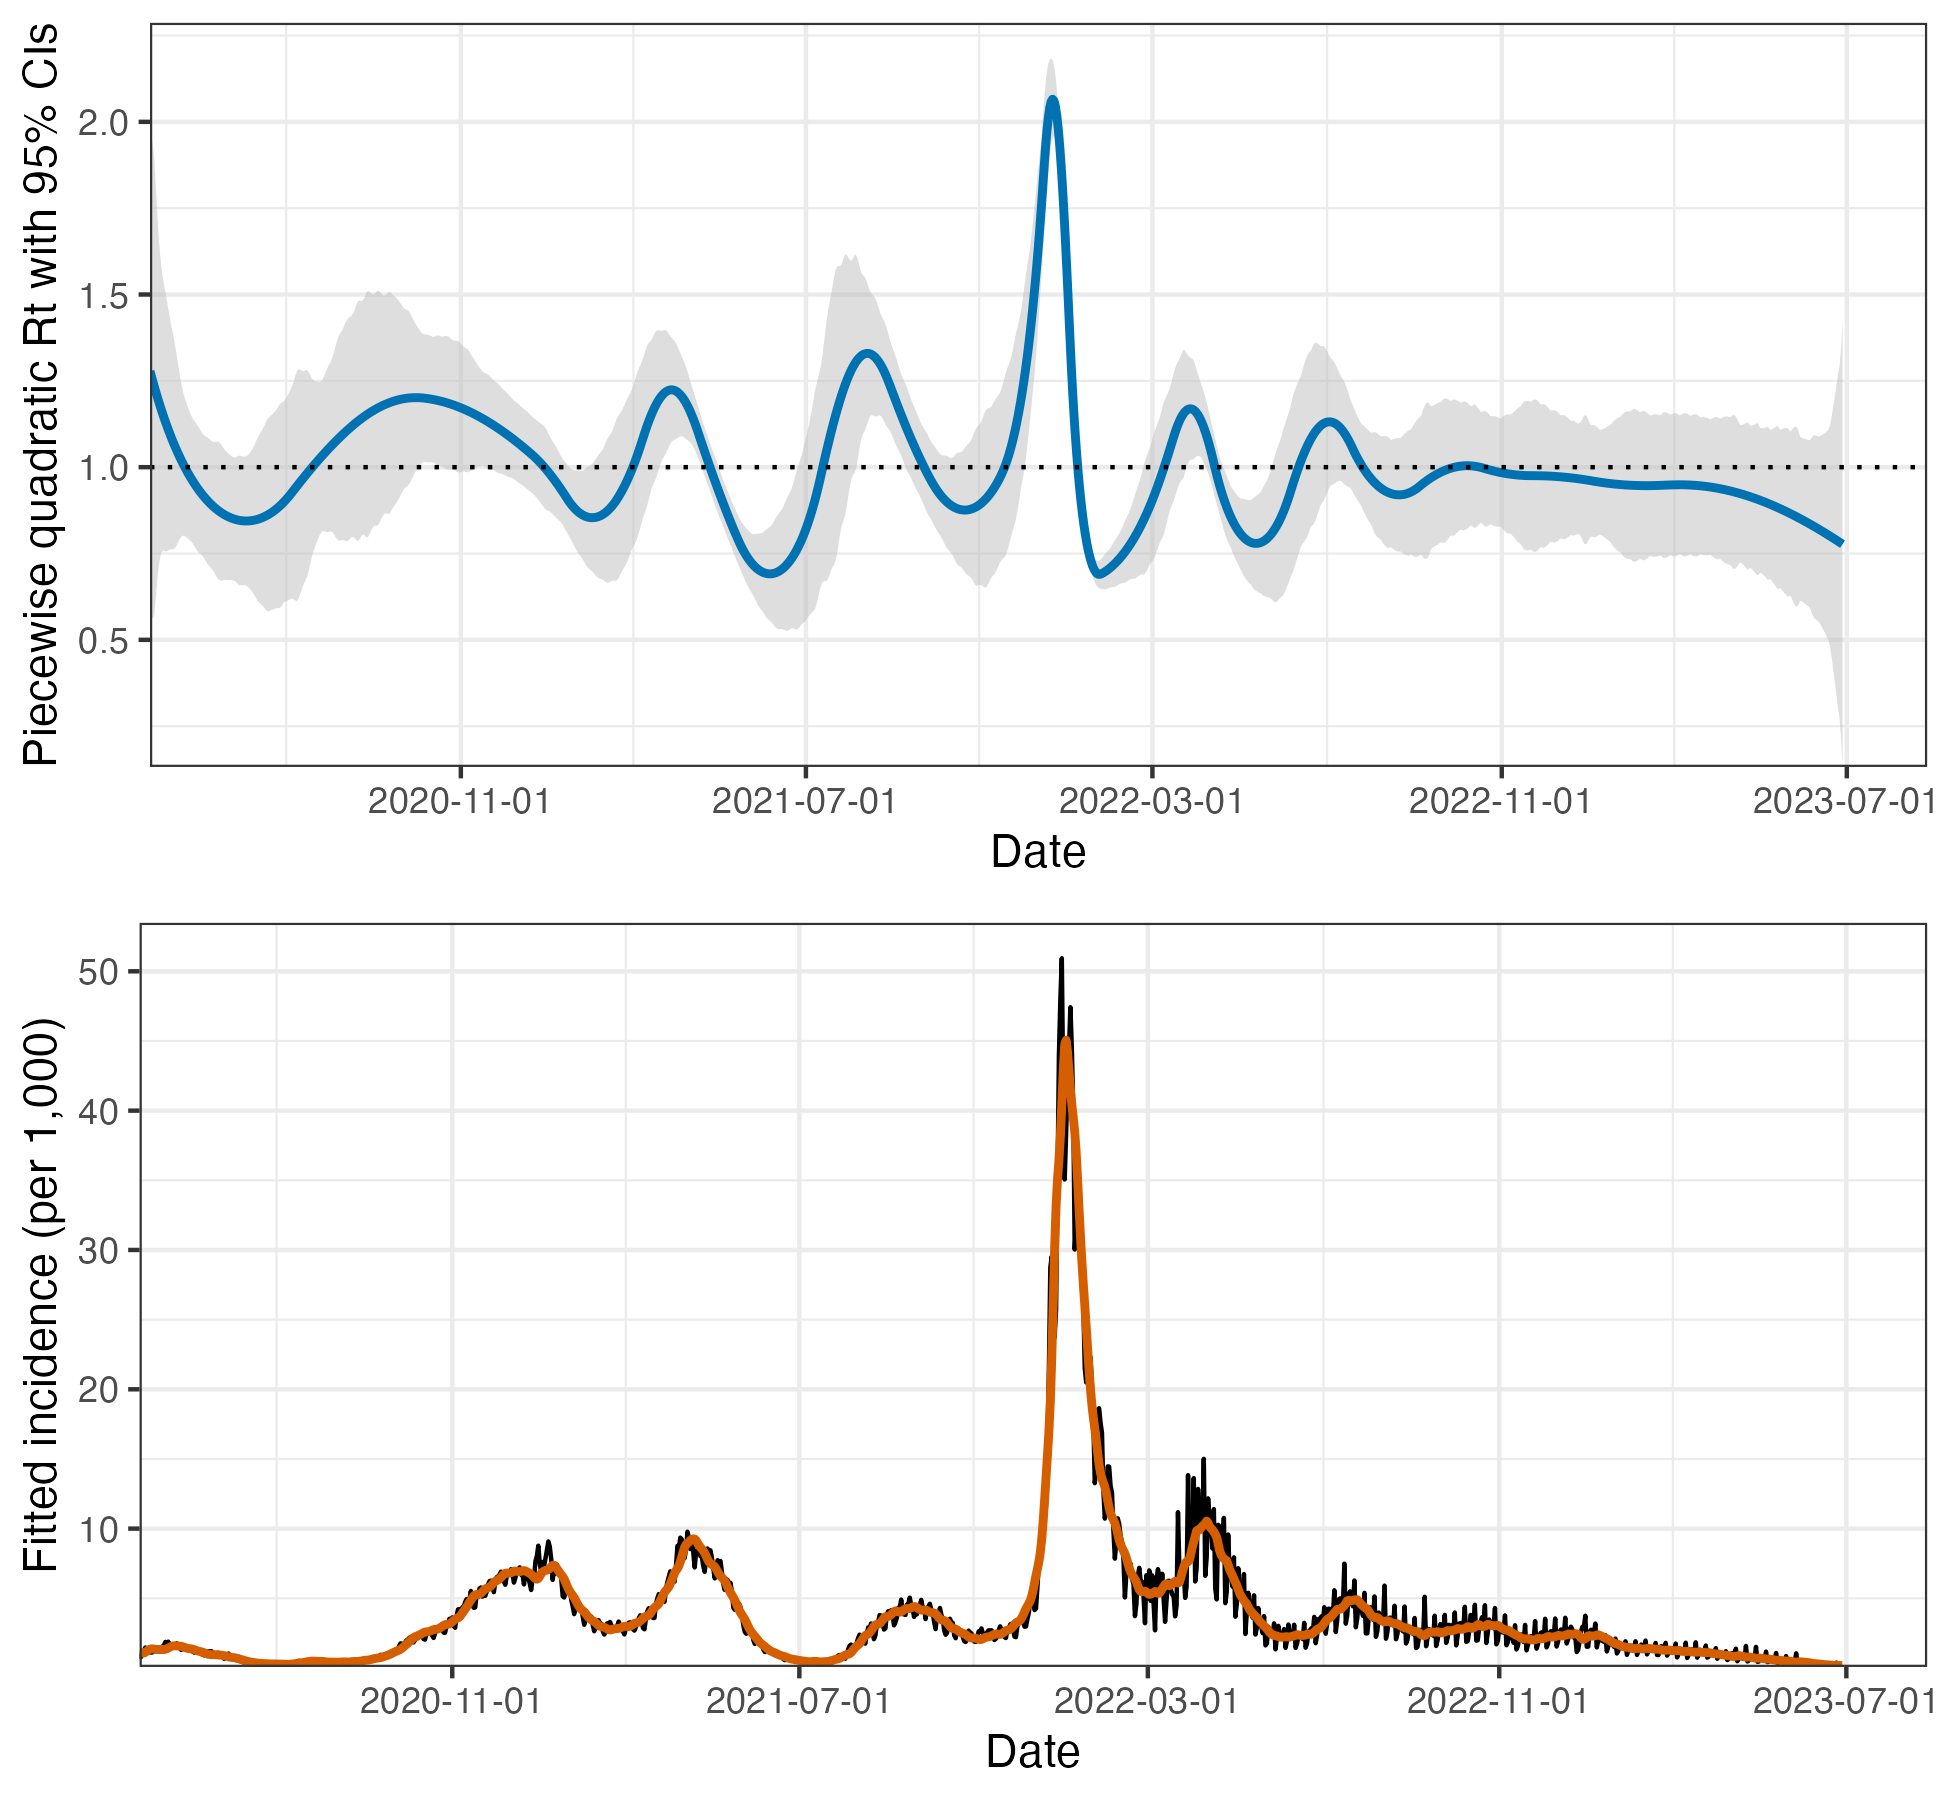
\includegraphics[width=.9\textwidth]{fig/intro-fig-new.png}
  \caption{A demonstration of effective reproduction number estimation 
  by \RtEstim\ and the corresponding predicted incident cases for the Covid-19 epidemic 
  in Canada during the period from March 28, 2020 to June 28, 2023. 
  In the top panel, the blue curve is the estimated piecewise
  quadratic $\calR_t$ and the gray ribbon is the corresponding 95\% confidence band. 
  The black curve in the bottom panel is the observed Covid-19 daily confirmed 
  cases, and the orange curve is the predicted incident cases
  corresponding to the estimated $\calR_t$.}
  \label{fig:intro-fig}
\end{figure}

While our approach is straightforward and requires little domain knowledge for
implementation, we also implement a number of refinements. 
We use a proximal Newton method to solve the convex optimization problem along
with warm starts to produce estimates efficiently, typically in a matter of 
seconds, even for long sequences of data. In a number of simulation experiments, 
we show empirically that our approach is more accurate than existing methods at 
estimating the true effective reproduction numbers. 


The manuscript proceeds as follows. We first introduce the methodology of
\RtEstim\ including the renewal equation and the development of Poisson
trend filtering estimator. We explain how this method could be interpreted from
the Bayesian perspective, connecting it to previous work in this context. We
provide illustrative experiments comparing our estimator to \EpiEstim\ and
\EpiLPS. We then apply our \RtEstim\ on the Covid-19 pandemic incidence in
British Columbia and the 1918 influenza pandemic incidence in the United States. 
Finally, we conclude with a discussion of the advantages and limitations of our 
approach and describe practical considerations for effective reproduction number
estimation.
